% !TEX TS-program = pdflatex
\documentclass[11pt]{article}

% -------------------- Packages --------------------
\usepackage[a4paper,margin=1in]{geometry}
\usepackage{amsmath,amssymb}
\usepackage[T1]{fontenc}
\usepackage{lmodern}
\usepackage{xcolor}
\usepackage{tcolorbox}
\tcbuselibrary{skins,breakable}
\usepackage{enumitem}
\usepackage{hyperref}
\usepackage{tikz}
\usetikzlibrary{calc}

\pagestyle{empty}

% -------------------- Dark Theme Colors --------------------
\definecolor{bg}{HTML}{000000}
\definecolor{pairbg}{HTML}{121212}
\definecolor{solbg}{HTML}{0A0A0A}
\definecolor{border}{HTML}{2A2A2A}
\definecolor{text}{HTML}{FFFFFF}
\definecolor{muted}{HTML}{C9CDD3}
\definecolor{gold}{HTML}{FFD700}
\definecolor{green}{HTML}{4ADE80}
\definecolor{cyan}{HTML}{38BDF8}

\pagecolor{bg}
\color{text}

\hypersetup{
  colorlinks=true,
  linkcolor=cyan,
  urlcolor=cyan
}

\setlength{\parindent}{0pt}
\setlength{\parskip}{10pt}

\setlist[itemize]{left=1.4em,itemsep=6pt,topsep=6pt}
\setlist[enumerate]{left=1.6em,itemsep=4pt,topsep=4pt}

% -------------------- tcolorbox Base --------------------
\tcbset{
  enhanced,
  breakable,
  arc=12pt,
  boxrule=0.8pt,
  left=16pt,right=16pt,top=12pt,bottom=12pt
}

\newtcolorbox{QAPair}[1]{%
  colback=pairbg,
  colbacklower=solbg,
  colframe=border,
  coltext=text,
  title=\textcolor{gold}{\bfseries #1},
  fonttitle=\bfseries,
  coltitle=text,
  segmentation style={draw=border, dashed, line width=0.6pt},
}

% Visible text inside this box (fix)
\newtcolorbox{QuickBox}{%
  colback=pairbg,
  colframe=cyan,
  coltext=text,
  fontupper=\color{text},
  borderline north={4pt}{0pt}{cyan},
  arc=14pt,
  boxrule=0.8pt
}

% Helper for step headings
\newcommand{\Step}[1]{\textcolor{muted}{\textbf{Step #1:}}}

% TikZ styles (kept minimal)
\tikzset{
  axis/.style={->, line width=0.9pt, draw=muted},
  poly/.style={line width=1.0pt, draw=cyan},
  midseg/.style={line width=1.0pt, draw=green},
  pt/.style={circle, fill=gold, inner sep=1.6pt},
  midpt/.style={circle, fill=green, inner sep=1.6pt},
  lab/.style={text=text, font=\small}
}

% ============================================================
\begin{document}

\begin{center}
{\LARGE\bfseries \textcolor{gold}{Exercise 7.2 --- Solutions}}\\[-2pt]
\end{center}

\begin{QuickBox}
{\color{cyan}\bfseries Quick formulas (useful)}\par\medskip
\begin{itemize}
\item \textbf{Midpoint of } $(x_1,y_1)$ \textbf{and } $(x_2,y_2)$:
\[
M\left(\frac{x_1+x_2}{2},\,\frac{y_1+y_2}{2}\right).
\]
\item \textbf{Distance between } $(x_1,y_1)$ \textbf{and } $(x_2,y_2)$:
\[
d=\sqrt{(x_2-x_1)^2+(y_2-y_1)^2}.
\]
\item \textbf{Diagonals bisect each other} $\Longleftrightarrow$ \textbf{their midpoints are the same.}
\item \textbf{Mid-segment theorem (triangle):} segment joining midpoints of two sides is \textbf{parallel} to the third side and has \textbf{half} its length.
\end{itemize}
\end{QuickBox}

% ============================================================
% Q1
\begin{QAPair}{Question 1 (i)}
\textcolor{gold}{\bfseries Question:} Find the midpoint of the line segment joining $(2,5)$ and $(6,9)$.\\
\tcblower
\textcolor{green}{\bfseries Answer:}
\[
\begin{aligned}
\Step{1}\;& M\left(\frac{x_1+x_2}{2},\,\frac{y_1+y_2}{2}\right)\\
\Step{2}\;&= \left(\frac{2+6}{2},\,\frac{5+9}{2}\right)= (4,7).
\end{aligned}
\]
\end{QAPair}

\begin{QAPair}{Question 1 (ii)}
\textcolor{gold}{\bfseries Question:} Find the midpoint of the line segment joining $(-1,0)$ and $(2,2)$.\\
\tcblower
\textcolor{green}{\bfseries Answer:}
\[
\begin{aligned}
\Step{1}\;& M=\left(\frac{-1+2}{2},\,\frac{0+2}{2}\right)\\
\Step{2}\;&= \left(\frac12,\,1\right).
\end{aligned}
\]
\end{QAPair}

\begin{QAPair}{Question 1 (iii)}
\textcolor{gold}{\bfseries Question:} Find the midpoint of the line segment joining $(1.4,-1.5)$ and $(2.6,3.5)$.\\
\tcblower
\textcolor{green}{\bfseries Answer:}
\[
\begin{aligned}
\Step{1}\;& M=\left(\frac{1.4+2.6}{2},\,\frac{-1.5+3.5}{2}\right)\\
\Step{2}\;&= \left(\frac{4.0}{2},\,\frac{2.0}{2}\right)=(2,1).
\end{aligned}
\]
\end{QAPair}

% ============================================================
% Q2
\begin{QAPair}{Question 2 (i)}
\textcolor{gold}{\bfseries Question:} In quadrilateral $ABCD$ with
$A(1,0)$, $B(5,2)$, $C(2,6)$, $D(-3,2)$,
$E,F,G,H$ are midpoints of $AB,BC,CD,DA$. Find coordinates of $E,F,G,H$.\\
\tcblower
\textcolor{green}{\bfseries Answer:}
\[
\begin{aligned}
\Step{1}\;&E=\text{midpoint of }A(1,0)\text{ and }B(5,2)
=\left(\frac{1+5}{2},\frac{0+2}{2}\right)=(3,1).\\
\Step{2}\;&F=\text{midpoint of }B(5,2)\text{ and }C(2,6)
=\left(\frac{5+2}{2},\frac{2+6}{2}\right)=\left(\frac72,4\right).\\
\Step{3}\;&G=\text{midpoint of }C(2,6)\text{ and }D(-3,2)
=\left(\frac{2+(-3)}{2},\frac{6+2}{2}\right)=\left(-\frac12,4\right).\\
\Step{4}\;&H=\text{midpoint of }D(-3,2)\text{ and }A(1,0)
=\left(\frac{-3+1}{2},\frac{2+0}{2}\right)=(-1,1).
\end{aligned}
\]
\end{QAPair}

\begin{QAPair}{Question 2 (ii)}
\textcolor{gold}{\bfseries Question:} Draw line segments $EF$, $FG$, $GH$ and $HE$ by joining the midpoints.\\
\tcblower
\textcolor{green}{\bfseries Answer:} A neat sketch (with points labelled) is shown below.
\[
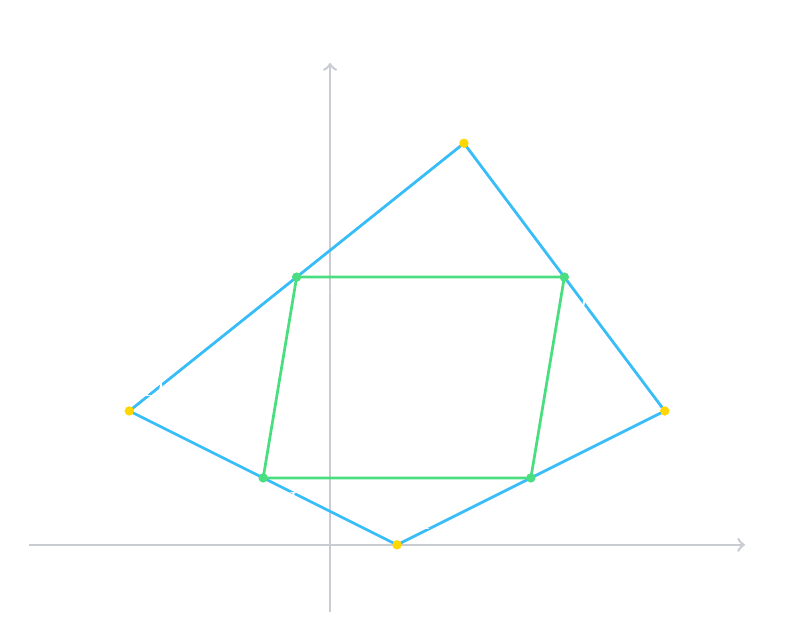
\begin{tikzpicture}[scale=0.85]
  % axes
  \draw[axis] (-4.5,0)--(6.2,0) node[lab, right] {$x$};
  \draw[axis] (0,-1)--(0,7.2) node[lab, above] {$y$};

  % points
  \coordinate (A) at (1,0);
  \coordinate (B) at (5,2);
  \coordinate (C) at (2,6);
  \coordinate (D) at (-3,2);

  \coordinate (E) at (3,1);
  \coordinate (F) at (3.5,4);
  \coordinate (G) at (-0.5,4);
  \coordinate (H) at (-1,1);

  % quadrilateral
  \draw[poly] (A)--(B)--(C)--(D)--cycle;

  % midpoint quadrilateral
  \draw[midseg] (E)--(F)--(G)--(H)--cycle;

  % plot points
  \foreach \P/\name in {A/A,B/B,C/C,D/D}{
    \fill[pt] (\P) circle (2pt);
    \node[lab] at ($( \P ) + (0.35,0.35)$) {$\name$};
  }
  \foreach \P/\name in {E/E,F/F,G/G,H/H}{
    \fill[midpt] (\P) circle (2pt);
    \node[lab] at ($( \P ) + (0.35,-0.35)$) {$\name$};
  }
\end{tikzpicture}
\]
\end{QAPair}

\begin{QAPair}{Question 2 (iii)}
\textcolor{gold}{\bfseries Question:} Find the lengths $EF$, $FG$, $GH$ and $HE$.\\
\tcblower
\textcolor{green}{\bfseries Answer:}
Using $d=\sqrt{(x_2-x_1)^2+(y_2-y_1)^2}$ with
$E(3,1)$, $F(\tfrac72,4)$, $G(-\tfrac12,4)$, $H(-1,1)$:
\[
\begin{aligned}
\Step{1}\;& EF=\sqrt{\left(\frac72-3\right)^2+(4-1)^2}
=\sqrt{\left(\frac12\right)^2+3^2}
=\sqrt{\frac14+9}
=\sqrt{\frac{37}{4}}=\frac{\sqrt{37}}{2}.\\[4pt]
\Step{2}\;& FG=\sqrt{\left(-\frac12-\frac72\right)^2+(4-4)^2}
=\sqrt{(-4)^2}=4.\\[4pt]
\Step{3}\;& GH=\sqrt{\left(-1+\frac12\right)^2+(1-4)^2}
=\sqrt{\left(-\frac12\right)^2+(-3)^2}
=\frac{\sqrt{37}}{2}.\\[4pt]
\Step{4}\;& HE=\sqrt{(3-(-1))^2+(1-1)^2}
=\sqrt{4^2}=4.
\end{aligned}
\]
So,
\[
EF=GH=\frac{\sqrt{37}}{2},\qquad FG=HE=4.
\]
\end{QAPair}

\begin{QAPair}{Question 2 (iv)}
\textcolor{gold}{\bfseries Question:} Guess the type of quadrilateral $EFGH$.\\
\tcblower
\textcolor{green}{\bfseries Answer:}
\[
\begin{aligned}
\Step{1}\;& \text{From (iii): } EF=GH \text{ and } FG=HE.\\
\Step{2}\;& \text{Also, } FG \text{ and } HE \text{ are both horizontal (same } y=4 \text{ and } y=1),\\
&\qquad\Rightarrow\; FG \parallel HE.\\
\Step{3}\;& \text{Slope}(EF)=\frac{4-1}{\frac72-3}=\frac{3}{\frac12}=6,\quad
\text{Slope}(GH)=\frac{1-4}{-1-(-\frac12)}=\frac{-3}{-\frac12}=6,\\
&\qquad\Rightarrow\; EF \parallel GH.
\end{aligned}
\]
Since both pairs of opposite sides are parallel, \textbf{$EFGH$ is a parallelogram.}
\end{QAPair}

% ============================================================
% Q3
\begin{QAPair}{Question 3}
\textcolor{gold}{\bfseries Question:} Check by using the midpoint formula whether the diagonals of trapezium $PQRS$
with $P(1,0)$, $Q(6,0)$, $R(7,4)$, $S(-1,4)$ bisect each other or not.\\
\tcblower
\textcolor{green}{\bfseries Answer:}
Diagonals are $PR$ and $QS$.
\[
\begin{aligned}
\Step{1}\;& \text{Midpoint of }PR:
M_{PR}=\left(\frac{1+7}{2},\,\frac{0+4}{2}\right)=(4,2).\\
\Step{2}\;& \text{Midpoint of }QS:
M_{QS}=\left(\frac{6+(-1)}{2},\,\frac{0+4}{2}\right)=\left(\frac52,2\right).\\
\Step{3}\;& M_{PR}\neq M_{QS}\;\Rightarrow\;\text{the diagonals do \textbf{not} bisect each other.}
\end{aligned}
\]
\end{QAPair}

% ============================================================
% Q4
\begin{QAPair}{Question 4}
\textcolor{gold}{\bfseries Question:} If vertices of a rhombus are
$A(-3,-1)$, $B(0,0)$, $C(1,3)$, $D(-2,2)$.
Show that its diagonals bisect each other. Also find the length of each diagonal.\\
\tcblower
\textcolor{green}{\bfseries Answer:}
Diagonals are $AC$ and $BD$.
\[
\begin{aligned}
\Step{1}\;& \text{Midpoint of }AC:
M_{AC}=\left(\frac{-3+1}{2},\,\frac{-1+3}{2}\right)=(-1,1).\\
\Step{2}\;& \text{Midpoint of }BD:
M_{BD}=\left(\frac{0+(-2)}{2},\,\frac{0+2}{2}\right)=(-1,1).\\
\Step{3}\;& M_{AC}=M_{BD}\;\Rightarrow\;\text{diagonals bisect each other.}\\[6pt]
\Step{4}\;& AC=\sqrt{(1-(-3))^2+(3-(-1))^2}
=\sqrt{4^2+4^2}=\sqrt{32}=4\sqrt{2}.\\
\Step{5}\;& BD=\sqrt{((-2)-0)^2+(2-0)^2}
=\sqrt{(-2)^2+2^2}=\sqrt{8}=2\sqrt{2}.
\end{aligned}
\]
So, \(\boxed{AC=4\sqrt2,\; BD=2\sqrt2}\).
\end{QAPair}

% ============================================================
% Q5
\begin{QAPair}{Question 5 (i)}
\textcolor{gold}{\bfseries Question:} In $\triangle ABC$ with $A(3,7)$, $B(-4,0)$, $C(4,0)$,
find the coordinates of midpoints $D$ of $AB$ and $E$ of $AC$.\\
\tcblower
\textcolor{green}{\bfseries Answer:}
\[
\begin{aligned}
\Step{1}\;& D=\left(\frac{3+(-4)}{2},\,\frac{7+0}{2}\right)=\left(-\frac12,\frac72\right).\\
\Step{2}\;& E=\left(\frac{3+4}{2},\,\frac{7+0}{2}\right)=\left(\frac72,\frac72\right).
\end{aligned}
\]
\end{QAPair}

\begin{QAPair}{Question 5 (ii)}
\textcolor{gold}{\bfseries Question:} Find $d(D,E)$ and $d(B,C)$.\\
\tcblower
\textcolor{green}{\bfseries Answer:}
\[
\begin{aligned}
\Step{1}\;& d(D,E)=\sqrt{\left(\frac72-\left(-\frac12\right)\right)^2+\left(\frac72-\frac72\right)^2}
=\sqrt{4^2+0}=4.\\
\Step{2}\;& d(B,C)=\sqrt{(4-(-4))^2+(0-0)^2}
=\sqrt{8^2}=8.
\end{aligned}
\]
So, \(\boxed{d(D,E)=4,\; d(B,C)=8}\).
\end{QAPair}

\begin{QAPair}{Question 5 (iii)}
\textcolor{gold}{\bfseries Question:} Find half of $d(B,C)$.\\
\tcblower
\textcolor{green}{\bfseries Answer:}
\[
\Step{1}\; \frac12\,d(B,C)=\frac12\cdot 8=4.
\]
\end{QAPair}

\begin{QAPair}{Question 5 (iv)}
\textcolor{gold}{\bfseries Question:} Compare the length of $DE$ and $BC$ and draw conclusion.\\
\tcblower
\textcolor{green}{\bfseries Answer:}
\[
\begin{aligned}
\Step{1}\;& d(D,E)=4,\quad d(B,C)=8 \;\Rightarrow\; d(D,E)=\frac12\,d(B,C).\\
\Step{2}\;& \text{Also, }B(-4,0)\text{ and }C(4,0)\Rightarrow BC \text{ is horizontal.}\\
&\qquad D\!\left(-\frac12,\frac72\right)\text{ and }E\!\left(\frac72,\frac72\right)\Rightarrow DE \text{ is also horizontal.}\\
\Step{3}\;& \Rightarrow\; DE \parallel BC \text{ and } DE=\frac12\,BC.
\end{aligned}
\]
\textbf{Conclusion:} The segment joining midpoints of two sides of a triangle is \textbf{parallel} to the third side and equals \textbf{half} of it.
\end{QAPair}

% ============================================================
% Q6
\begin{QAPair}{Question 6}
\textcolor{gold}{\bfseries Question:} Hassan starts from a point on $x$-axis and Ali from a point on $y$-axis,
each at a distance of $6$ units from origin. They reach the same target point $C$ after covering an equal distance.
Find coordinates of (i) starting points of Hassan and Ali, (ii) target point $C$.\\
\tcblower
\textcolor{green}{\bfseries Answer:}
\[
\begin{aligned}
\Step{1}\;& \text{On the positive }x\text{-axis, }6\text{ units from origin: }H=(6,0).\\
\Step{2}\;& \text{On the positive }y\text{-axis, }6\text{ units from origin: }A=(0,6).\\
\Step{3}\;& \text{Equal distances }HC=AC \text{ and (as in the figure) }C \text{ lies on segment }HA,\\
&\qquad\Rightarrow\; C \text{ is the midpoint of }H(6,0)\text{ and }A(0,6).\\
\Step{4}\;& C=\left(\frac{6+0}{2},\,\frac{0+6}{2}\right)=(3,3).
\end{aligned}
\]
So, \(\boxed{\text{Hassan }(6,0),\; \text{Ali }(0,6),\; C(3,3)}\).
\[
\begin{tikzpicture}[scale=0.8]
  \draw[axis] (-1,0)--(7.2,0) node[lab,right] {$x$};
  \draw[axis] (0,-1)--(0,7.2) node[lab,above] {$y$};

  \coordinate (H) at (6,0);
  \coordinate (A) at (0,6);
  \coordinate (C) at (3,3);

  \draw[poly] (A)--(H);
  \fill[pt] (H) circle (2pt) node[lab, below right] {Hassan $(6,0)$};
  \fill[pt] (A) circle (2pt) node[lab, above left] {Ali $(0,6)$};
  \fill[midpt] (C) circle (2pt) node[lab, above right] {$C(3,3)$};
\end{tikzpicture}
\]
\end{QAPair}

% ============================================================
% Q7
\begin{QAPair}{Question 7 (i)}
\textcolor{gold}{\bfseries Question:} Label the missing coordinates of the vertices of the square $OLMN$
(given $L(3,0)$ and $O$ at origin).\\
\tcblower
\textcolor{green}{\bfseries Answer:}
Since $O=(0,0)$ and $L=(3,0)$, the side length is $3$ units, so the top vertices have $y=3$:
\[
\boxed{O(0,0),\; L(3,0),\; M(3,3),\; N(0,3).}
\]
\end{QAPair}

\begin{QAPair}{Question 7 (ii)}
\textcolor{gold}{\bfseries Question:} Label the missing coordinates of the vertices of rectangle $ABCD$
(given $B(0,2)$ and $D(-4,0)$; $A$ lies at the origin on the figure).\\
\tcblower
\textcolor{green}{\bfseries Answer:}
$A$ is at the origin, so $A=(0,0)$. With $B=(0,2)$, the top side has $y=2$. With $D=(-4,0)$, the left side has $x=-4$.
Hence the remaining vertex is $C=(-4,2)$:
\[
\boxed{A(0,0),\; B(0,2),\; C(-4,2),\; D(-4,0).}
\]
\end{QAPair}

\end{document}
